\documentclass{article}

\usepackage{preamble}

\title{Causality in Event Structure}
\author{Amir Hossein Seyhani}
\date{June 2022}

\begin{document}

\maketitle

\tableofcontents
\pagebreak

\section{Introduction}

\section{Preliminaries}
\subsection{Event Structure}
\begin{definition}[Event Structure]
    An event structure is a triple $E = (\mathcal{E},\#,\vdash)$ where:
    \begin{enumerate}
        \item $\mathcal{E}$ is a set of events
        \item \# is a binary symmetric, irreflexive relation on $\mathcal{E}$,
              the conflict relation.
              We shall write $Con$ for the set of conflict-free subsets of $\mathcal{E}$,
              i.e. those finite subsets $X \subseteq \mathcal{E}$ for which:
              $\forall e,e' \in X . \neg (e\#e')$
        \item $\vdash \subseteq Con \times \mathcal{E}$ is the enabling relation which satisfies:
              $ X \vdash e \ \& \ X \subseteq Y \in Con \Rightarrow Y \vdash e$
    \end{enumerate}

\end{definition}
\begin{notion}
    In an event structure we shall write $\doublevee$ for the reflexive conflict relation by which we mean
    that $e\doublevee e'$ in an event structure iff either $e\#e'$ or $e=e'$.
    With this notion instead of describing the conflict-free sets of an event structure
    as those sets $X$ such that
    \begin{align*}
        \forall e,e' \in X. \neg(e\#e')
    \end{align*}
    we can say they are those sets $X$ for which:
    \begin{align*}
        \forall e,e' \in X. e\doublevee e' \Rightarrow e=e'
    \end{align*}
\end{notion}

\begin{notion}
    For any event structure we can define the minimal enabling relation $\vdash_{min}$ by:
    \begin{align*}
        X \vdash_{min} e \iff X \vdash e \amp
        ( \forall Y \subseteq X . Y \vdash e \Rightarrow Y = X )
    \end{align*}
    Then for any event structure:
    \begin{align*}
        Y \vdash e \Rightarrow \exists X \subseteq Y . X \vdash_{min} e
    \end{align*}
\end{notion}

\begin{definition}[Configuration]
    \label{conf}
    Let $E = (\mathcal{E},\#,\vdash)$ be an event structure.
    Define a configuration of $E$ to be a subset of events $x \subseteq \mathcal{E}$ which is
    \begin{enumerate}
        \item conflict-free: $x \in Con$
        \item secured: $\forall e \in x \exists e_0,...,e_n \in x. e_n = e \ \& \
                  \forall i \leq n. \s{e_0,...,e_{i-1}} \vdash e_i$
    \end{enumerate}
\end{definition}
The set of all configurations of an event structure is written as $\mathcal{F(E)}$.
It is helpful to unwrap condition (2) a little. It says an event $e$ is secured in a set $x$
iff there is a sequence of events $e_0,...,e_n = e$ in $x$ such that:
\begin{align*}
    \emptyset \vdash e_0, \s{e_0} \vdash e_1, ..., \s{e_0,...,e_{i-1}} \vdash e_i,...,
    \s{e_0,...,e_{n-1}} \vdash e_n.
\end{align*}
We call such a sequence $e_0,e_1,...,e_n = e$ a \emph{securing} for $e$ in $x$.
We use $X \subseteq_{fin} Y$ to mean $X$ is a finite subset of $Y$.

\begin{example}
    Event structures can exhibit non-determinism, or conflict.
    Consider the event structure with two events 0,1 in which
    $\emptyset \vdash 0$ and $\emptyset \vdash 1$,
    $\s{0},\s{1} \in Con$ and yet $\s{0,1} \not \in Con$.
    We illustrate configurations of event structures using the Hasse diagram of
    the partial order of configurations ordered by inclusion:
    \begin{center}
        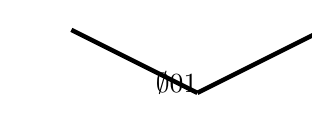
\begin{tikzpicture}[scale=0.8]
            \crd{0}{0}{$\emptyset$}
            \crd{-2}{1}{$\s{0}$}
            \crd{2}{1}{$\s{1}$}
            \draw [ultra thick] (0,0) -- (2,1);
            \draw [ultra thick] (0,0) -- (-2,1);
        \end{tikzpicture}
    \end{center}
    Non-determinism appears as branching in the partial order of configurations.
\end{example}

\begin{example}
    Event structures can exhibit parallelism, or concurrency.
    The event structure with two events 0,1 in which
    $\emptyset \vdash 0$ and $\emptyset \vdash 1$,
    $\s{0},\s{1} \in Con$ and this time $\s{0,1} \in Con$,
    has the configurations of the form:
    \begin{center}
        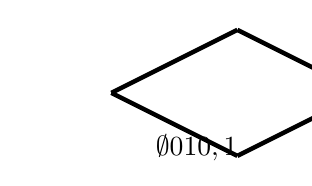
\begin{tikzpicture}[scale=0.8]
            \crd{0}{0}{$\emptyset$}
            \crd{-2}{1}{$\s{0}$}
            \crd{2}{1}{$\s{1}$}
            \crd{0}{2}{$\s{0,1}$}
            \draw [ultra thick] (0,0) -- (2,1);
            \draw [ultra thick] (0,0) -- (-2,1);
            \draw [ultra thick] (-2,1) -- (0,2);
            \draw [ultra thick] (2,1) -- (0,2);
        \end{tikzpicture}
    \end{center}
    Concurrency of events appears as a little square in the partial order of configurations.
\end{example}

\begin{example}
    Consider two parallel switches in a circuit where they are connected
    to a light bulb.
    An event may be enabled in more than one way even in a single configuration.
    Assume initially both switches are open.
    Closing either one enables the event of the bulb lighting up.
    The configurations have the form:

    \begin{center}
        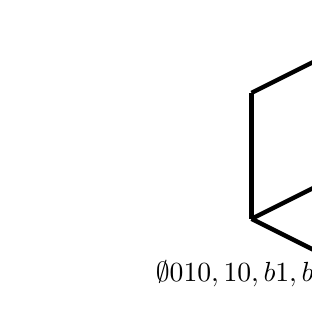
\begin{tikzpicture}[scale=0.8]
            \crd{0}{0}{$\emptyset$}
            \crd[left]{-2}{1}{$\s{0}$}
            \crd[right]{2}{1}{$\s{1}$}
            \crd[right]{0}{2}{$\s{0,1}$}
            \crd{-2}{3}{$\s{0,b}$}
            \crd{2}{3}{$\s{1,b}$}
            \crd{0}{4}{$\s{0,1,b}$}
            \draw [ultra thick] (0,0) -- (2,1);
            \draw [ultra thick] (0,0) -- (-2,1);
            \draw [ultra thick] (-2,1) -- (0,2);
            \draw [ultra thick] (2,1) -- (0,2);
            \draw [ultra thick] (-2,1) -- (-2,3);
            \draw [ultra thick] (0,2) -- (0,4);
            \draw [ultra thick] (2,1) -- (2,3);
            \draw [ultra thick] (-2,3) -- (0,4);
            \draw [ultra thick] (2,3) -- (0,4);
        \end{tikzpicture}
    \end{center}
\end{example}

We look for a special class of event structures for which there is a
partial order of causal dependency on each configuration.
This can not be done so obviously for all event structures.
Consider the event structure of the previous example in which
the event $b$ causally depends not on a unique set of events
but rather on either the occurrence of 0 or on the occurrence of 1.
It is incorrect to say $b$ causally depends on both 0 and 1 because
the occurrence of only one of them enables the occurrence of $b$.
The difficulty arises because there is a configuration $\s{0,1,b}$
in which there is an event $b$ which is not enabled by a unique minimal
set of event occurrences.
We can rule out such possibilities by insisting event structures
satisfy the following stability axiom.

\begin{definition}[Stable Event Structure]
    Let $E = (\mathcal{E},\#,\vdash)$ be an event structure. Say $E$ is stable if it satisfies the following axiom:
    \begin{align*}
        X \vdash e \ \& \ Y \vdash e \ \& \ X \cup Y \cup \{e\} \in Con \Rightarrow X \cap Y \vdash e
    \end{align*}
\end{definition}

\begin{example}
    Let $E$ be the event structure with events $\s{0,1,2}$
    with consistency predicate the least one such that:
    \begin{align*}
        \s{0,1},\s{0,2},\s{1,2} \in Con
    \end{align*}
    so $\s{0,1,2} \not \in Con$, and enabling relation the least
    one such that
    \begin{align*}
        \emptyset \vdash 0, \emptyset \vdash 1,
        \s{0} \vdash 2, \s{1} \vdash 2
    \end{align*}
    Then $E$ is a stable event structure and the configurations
    $\mathcal{F}(E)$ have the form
    \begin{center}
        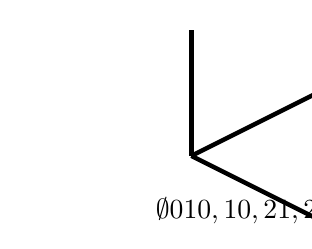
\begin{tikzpicture}[scale=0.8]
            \crd{0}{0}{$\emptyset$}
            \crd[left]{-2}{1}{$\s{0}$}
            \crd[right]{2}{1}{$\s{1}$}
            \crd[right]{0}{2}{$\s{0,1}$}
            \crd{-2}{3}{$\s{0,2}$}
            \crd{2}{3}{$\s{1,2}$}
            \draw [ultra thick] (0,0) -- (2,1);
            \draw [ultra thick] (0,0) -- (-2,1);
            \draw [ultra thick] (-2,1) -- (0,2);
            \draw [ultra thick] (2,1) -- (0,2);
            \draw [ultra thick] (-2,1) -- (-2,3);
            \draw [ultra thick] (2,1) -- (2,3);
        \end{tikzpicture}
    \end{center}
\end{example}

The stability axiom ensures that an event in a configuration is
enabled in an essentially unique way.
Assume $e$ belongs to a configuration $x$ of a stable event structure.
Suppose $X \vdash e$ and $X \subseteq x$.
Then $X \cup \s{e} \in Con$, the enabling $X\vdash e$ is consistent.
Take
\begin{align*}
    X_0 = \cap \s{Y | Y \subseteq X \amp Y \vdash e}
\end{align*}
Because $X$ is finite this is an intersection of a finite number of
sets and we see by the stability axiom that $X_0 \vdash e$.
Moreover $X_0$ is the unique minimal subset of $X$ which enables $e$.
Thus for stable event structures we have:
\begin{align*}
    Y \vdash e \amp Y \cup \s{e} \in Con \Rightarrow
    \exists ! X \subseteq Y.X \vdash_{min} e
\end{align*}
It follows that for stable event structures
\begin{align*}
    X \vdash_{min} e \amp Y \vdash_{min} \amp
    X \cup Y \cup e \in Con \Rightarrow X = Y
\end{align*}

\begin{theorem}
    Let $E = (\mathcal{E}, \#, \vdash)$ be an event structure.
    Let $x = \s{e_1,e_2,...,e_m}$ be a conflict-free subset of $\mathcal{E}$.
    Then $x$ is secured according to the definition \ref{conf} iff
    there exists an event $e_{i_n} \in x$ with a securing sequence $e_{i_1},e_{i_2},...,e_{i_{m-1}}$.

    \begin{proof}
        Assume that $x$ is secured. 
    \end{proof}

\end{theorem}

\begin{definition}
    Let $E_0 = (\mathcal{E}_0,\#_0,\vdash_0)$ and $E_1 = (\mathcal{E}_1,\#_1,\vdash_1)$
    be event Structures. Define
    \begin{align*}
        E_0 \trianglelefteq E_1 \iff & \mathcal{E}_0 \subseteq \mathcal{E}_1,                                          \\
                                     & \forall e,e'. e\#_0e'  \iff e,e' \in \mathcal{E}_0 \ \& \ e\#_1 e' \text{ and } \\
                                     & \forall X,e.X\vdash_0 e  \iff X \subseteq \mathcal{E}_0
        \ \& \ e \in \mathcal{E}_0\ \& \ X \vdash_1 e
    \end{align*}
    In this case say $E_0$ is a substructure of $E_1$.
\end{definition}

\begin{definition}[Restriction]
    Let $E = (\mathcal{E},\#,\vdash)$ be an event structure.
    Let $A \subseteq \mathcal{E}$.
    Define the restriction of $E$ to $A$ to be
    \begin{align*}
        E \lceil A = (A,\#_A,\vdash_A)
    \end{align*}
    where
    \begin{align*}
        X \in Con_A \iff X \subseteq A \ \& \ X \in Con \\
        X \vdash_A e \iff X \subseteq A \ \& \ e \in A \ \& \ X \vdash e
    \end{align*}
\end{definition}

\begin{definition}
    Let $a$ be an event.
    For an event structure $E = (\mathcal{E},\#,\vdash)$ define $aE$ to be the event structure $(\mathcal{E'},\#',\vdash')$ where:
    \begin{align*}
         & \mathcal{E'} = \s{(0,a)} \cup \s{(1,e)|e \in \mathcal{E}},                                                   \\
         & e_0' \#' e_1'  \iff \exists e_0,e_1.e_0' = (1,e_0)
        \ \& \ e_1' = (1,e_1) \ \& \ e_0 \# e_1                                                                         \\
         & X \vdash' e' \iff e' = (0,a) \text{ or } [e' = (1,e_1) \ \& \ (0,a)\in X \ \& \ \s{e|(1,e)\in X} \vdash e_1]
    \end{align*}
\end{definition}

\begin{definition}
    A labelled event structure consists of $(\mathcal{E},\#,\vdash,L,l)$ where
    $(\mathcal{E},\#,\vdash)$ is an event structure, $L$ is a set of labels,
    not including the element *, and $l$ is a function $l: \mathcal{E} \rightarrow L$
    from its events to its labels.
\end{definition}
\begin{notion}
    We write $(a_1,a_2,...,a_{n-1},a_n)$ to denote the event:
    \begin{align*}
        e = (a_1,(a_2,(a_3,...(a_{n-1},a_n))))
    \end{align*}
\end{notion}

\subsection{Causal Model}

A signature $\mathcal{S}$ is a tuple $(\mathcal{U},\mathcal{V},\mathcal{R})$,
where $\mathcal{U}$ is a set of exogenous variables, $\mathcal{V}$
is a set of endogenous variables, and $R$ associates with every variable
$Y\in \mathcal{U}\cup \mathcal{V}$ a nonempty set $\mathcal{R}(Y)$ of possible values for $Y$.
A causal model (or structural model) over signature $S$ is a tuple
$M=(\mathcal{S},\mathcal{F})$, where $\mathcal{F}$ associates with
each variable $X \in \mathcal{V}$ a function denoted $F_X$ such that
$F_X: (\times_{U\in \mathcal{U}}\mathcal{R}(U))\times (\times_{Y\in\mathcal{V}-\{X\}}\mathcal{R}(Y))\rightarrow \mathcal{R}(X)$.

$F_X$ determines the value of $X$ given the values of all the other variables
in $\mathcal{U}\cup \mathcal{V}$.
For example, if $F_X(Y,Z,U)=Y+U$ (which we usually write as $X = Y + U$),
then if $Y=3$ and $U=2$, then $X = 5$, regardless of how $Z$ is set.
These equations can be thought of as representing processes (or mechanisms) by which values are assigned to variables. Hence, like physical laws, they support a counterfactual interpretation.
For example, the equation above claims that in the context $U=u$, if $Y$ were 4, then $X$ would be $u+4$ (which we write as $(M,u) \models [Y\leftarrow 4](X = u + 4))$, regardless of what values X, Y, and Z actually take in the real world.


The function $\mathcal{F}$ defines a set of (\textit{modifiable}) \textit{structural equations} relating to the values of the variables.

\subsection{Definition of Actual Cause}
Given a signature $S= (\mathcal{U},\mathcal{V},\mathcal{R})$, a formula of the form $X =x$, for $X \in \mathcal{V}$ and $x \in \mathcal{R}(X)$, is called a \textit{primitive event}.
A \textit{basic causal formula} is one of the form $[Y_1 \leftarrow y_, ..., Y_l\leftarrow y_k]\varphi$, where $\varphi$ is a Boolean combination of primitive events, $Y_1,...,Y_k$ are distinct variables in $\mathcal{V}$, and $y_i \in \mathcal{R}(Y_i)$.
Such a formula is abbreviated as $[\vec{Y}\leftarrow\vec{y}]\varphi$.
A \textit{causal formula} is a Boolean combination of basic causal formulas.
A causal formula $\psi$ is true or false in a causal model, given a context.
We write $(M,\vec u)\models \psi$ if $\psi$ is true in causal model $M$ given context $\vec u$.
$(M,\vec u)\models [\vec Y\leftarrow \vec y](X=x)$ if the variable $X$ has value $x$ in the unique solution to the equation in $M_{\vec{Y} \leftarrow \vec{y}}$ in context $\vec u$.
The context and structural equations are given.
They encode the background knowledge.
All relevant events are known.
The only question is picking out which of them are the cause of $\varphi$ or, alternatively, testing whether a given set of events can be considered the cause of $\varphi$.
The types of events that we allow as actual causes are ones of the form $X_1 = x_1 \wedge ... \wedge X_k=x_k$-- that is, conjunctions of primitives events.
We abbreviate this as $\vec X = \vec x$.
\\
\\
\textbf{Definition 1:} $\vec X = \vec x$ is an actual cause of $\varphi$ in $(M,\vec u)$ if the following three conditions hold:
\begin{itemize}
    \item  \textbf{AC1.} $(M,\vec u)\models (\vec X = \vec x) \wedge \varphi$.
          (both $\vec X = \vec x$ and $\varphi$ are true in actual world)
    \item  \textbf{AC2. }There exists aa partition $(\vec Z, \vec W)$ of $\mathcal{V}$ with $\vec X \subseteq \vec Z$ and some setting $(\vec x',\vec w')$ of the variables in $(\vec X,\vec W)$ such that if $(M,\vec u)\models \vec Z = z^*$ for all $Z\in \vec Z$, then both of the following conditions hold:

          (a) $(M,\vec u)\models[\vec X \leftarrow \vec x', \vec W \leftarrow \vec w']\neg \varphi$.

          (b) $(M,\vec u)\models[\vec X\leftarrow \vec x, \vec W' \leftarrow \vec w', \vec Z'\leftarrow \vec z^*]\varphi$ for all subsets $\vec W'$ of $\vec W$ and all subsets $Z'$ of $\vec Z$.

    \item  \textbf{AC3.} $\vec X$ is minimal; no subset of $\vec X$ satisfies conditions $AC1$ and $AC2$.
\end{itemize}
We call the tuple $(\vec W, \vec w,x')$ a witness to the fact that $\vec X=\vec x$ is a cause of $\varphi$.

\section{Semantics of Communicating Processes}
One use of event structure is to give a denotational semantics of language of parallel
processes which reflects the parallelism in processes as causal independence between events.
The nature of the events, how they interact with the environment,
is specified in the language by associating each event with a label from the synchronization
algebra $L$.
The language we shall use is one where processes communicate by events of synchronization
with no value passing.
Its syntax has the form:
\begin{align*}
    p ::= nil | \alpha p | p_0 + p_1 | p_0 \times p_1 | p\lceil \Lambda | p[\Xi] | x | recx.p
\end{align*}
where $x$ is in some set of variables $X$ over processes, $\alpha$ is a label,
$\Lambda$ is a subset of labels, in $p[\Xi]$ the symbol $\Xi$ denotes a relabelling function between
two sets of labels.

Informally, the product $p_0 \times p_1$ is a form of parallel composition which introduces
arbitrary events of synchronization between process.
Unwanted synchronizations can be restricted away with the help of the restriction operation
$p\lceil \Lambda$ and the existing events renamed with the relabelling operation $p[\Xi]$.
So in this way we can define specialized parallel compositions of the kind that appear in
CCS and CSP, for example.
To explain formally the behavior of the constructs in the language we describe them as
constructions on labelled event structures, so a closed process term in this language is to
denote a \textbf{stable event structure} but where the events are labelled.

\subsection{Nil}
The term $nil$ represents the $nil$ process which has stopped and refuses to perform any event;
it will denoted by the empty labelled event structure $(\emptyset,\emptyset,\emptyset,\emptyset,\emptyset)$
no events, no labels.

\subsection{Prefix}

\begin{definition}
    Let $(\mathcal{E},L,l)$ be a labelled event structure.
    Let $\alpha$ be a label.
    Define $\alpha(\mathcal{E},L,l)$ to be a labelled event structure $(\alpha \mathcal{E},L',l')$
    with labels:
    \begin{align*}
        L' = \s{\alpha} \cup L
    \end{align*}
    and
    $$
        l'(e') = \begin{cases}
            \alpha & \text{if } e' = (0,\alpha) \\
            l(e)   & \text{if } e' = (1,e)
        \end{cases}
    $$
    for all $e' \in \mathcal{E'}$.
\end{definition}
The configurations of $\alpha E$, a prefixed labeled event structure,
have the simple and expected characterization.
(By $\mathcal{F}(E)$ of a labeled event structure $E$ we shall understand the set
of configurations of the underlying event structure)

\begin{proposition}

    Let $E$ be a labelled event structure. Let $\alpha$ be a label.
    \begin{align*}
        x \in \mathcal{F}(\alpha E) \iff x = \emptyset \text{ or }
        [(0,\alpha)\in x \amp \s{e | (1,e)\in x} \in \mathcal{F}(E)]
    \end{align*}

\end{proposition}

\subsection{Sum}
A sum $p_0 + p_1$ behaves like $p_0$ or $p_1$; which branch of a sum is followed will
often be determined by the context and what kinds of events the process is restricted to.

\begin{definition}
    Let $E_0 = (\mathcal{E}_0,\#_0,\vdash_0,L_0,l_0)$ and
    $E_1 = (\mathcal{E}_1,\#_1,\vdash_1,L_1,l_1)$ be labelled event structures.
    Their sum $E_0 + E_1$, is defined to be the structure $(\mathcal{E},\#,\vdash,l)$
    with events $\mathcal{E} = \s{(0,e)|e \in \mathcal{E}_0} \cup \s{(1,e)|e \in \mathcal{E}_1}$,
    the disjoint union of sets $\mathcal{E}_0$ and $\mathcal{E}_1$,
    with injections $\iota_k: \mathcal{E}_k \rightarrow \mathcal{E}$, given by
    $\iota_k(e) = (k,e)$, for $k=0,1$, conflict relation
    \begin{align*}
        e \# e' \iff & \exists e_0,e_0'. e = \iota_0(e_0)
        \amp e' = \iota_0(e_0') \amp e_0 \#_0e_0'                         \\
                     & \text{or } \exists e_1,e_1'. e = \iota_1(e_1) \amp
        e' = \iota_1(e_1') \amp e_1 \#_1 e_1'                             \\
                     & \text{or } \exists e_0,e_1.(e=\iota_1(e_0)
        \amp e' =\iota_1(e_1)) \text{ or }
        (e'=\iota_1(e_0) \amp e =\iota_1(e_1))
    \end{align*}
    and enabling relation
    \begin{align*}
        X \vdash e \iff & X \in Con \amp e \in \mathcal{E} \amp                       & \\
                        & (\exists X_0 \in Con_0,e_0 \in \mathcal{E}_0.X = \iota_0X_0
        \amp e = \iota_0(e_0) \amp X_0 \vdash_0 e_0) \text{ or }                        \\
                        & (\exists X_1 \in Con_1,e_1 \in \mathcal{E}_1.X = \iota_1X_1
        \amp e = \iota_1(e_1) \amp X_1 \vdash_1 e_1)                                    \\
    \end{align*}
    We define the set of labels as $L_0 \cup L_1$ and the labelling function as:
    $$
        l(e) = \begin{cases}
            l_0(e_0) & \text{ if } e = \iota_0(e_0) \\
            l_1(e_1) & \text{ if } e = \iota_1(e_1)
        \end{cases}
    $$
\end{definition}
The configurations of a sum are obtained from copies of the configurations of the components
identified at their empty configurations.

\begin{proposition}

    Let $E_0$ and $E_1$ be labelled event structures.
    \begin{align*}
        x \in \mathcal{F}(E_0+E_1) \iff (\exists x_0 \in \mathcal{F}(E_0).x=\iota_0x_0)
        \text{ or } (\exists x_1 \in \mathcal{F}(E_1).x=\iota_1x_1)
    \end{align*}

\end{proposition}

\subsection{Product}

A product process $p_0 \times p_1$ behaves like $p_0$ and $p_1$ set in parallel.
Their events of synchronization are those pairs of events $(e_0,e_1)$, one from each process;
if $e_0$ is labelled $\alpha_0$ and $e_1$ is labelled $\alpha_1$ the synchronization event is
then labelled $(\alpha_0,\alpha_1)$.
Events need not to synchronize however; an event in one component may not synchronize with
any event in the other.
We shall use events of the form $(e_0,*)$ to stand for the occurrence of an event $e_0$
from one component unsynchronized with any event of the other.
Such an event will be labelled by $(\alpha_0,*)$ where $\alpha_0$ is the original label of $e_0$
and * is a sort of undefined.

In fact we shall often want to take the first or second coordinates of such paris and,
of course, this could give the value * which we think of as undefined,
so that, in effect, we are working with partial functions with * understood to be undefined.
We can keep expressions tidier by adopting some conventions about how to treat this undefined value
when it appears in expressions and assertions.
\begin{align*}
     & \Theta(e) \in X \Rightarrow \Theta(e) \text{is defined, and }                                      \\
     & \Theta(e) = \Theta(e') \Rightarrow \Theta(e) \text{is defined } \amp \Theta(e')\text{ is defined}.
\end{align*}
We adopt a similar strict interpretation for function application.
So if $f$ is a function applied to some value, denoted by $a$, the $f(a)$ is undefined (gives *)
if $a$ is undefined.
As usual we represent the image of a set under a partial function by
\begin{align*}
    \Theta X = \s{\Theta(e)|e \in X \amp \Theta(e) \text{ is defined}}
\end{align*}

\begin{definition}

    Let $E_0 = (\mathcal{E}_0,\#_0,\vdash_0,L_0,l_0)$ and $E_1 = (\mathcal{E}_1,\#_1,\vdash_1,L_1,l_1)$
    be labelled event structures.
    Define their product $E_0 \times E_1$ to be the structure $E = (\mathcal{E},\#,\vdash,L,l)$
    consisting of events $\mathcal{E}$ of the form
    \begin{align*}
        \mathcal{E}_0 \times_* \mathcal{E}_1 =
        \s{(e_0,*)|e_0 \in \mathcal{E}_0}
        \cup \s{(*,e_1)|e_1 \in \mathcal{E}_1}
        \cup \s{(e_0,e_1)| e_0 \in \mathcal{E}_0 \amp e_1 \in \mathcal{E}_1}
    \end{align*}
    with projections $\pi_i : \mathcal{E} \rightarrow_* \mathcal{E}_i$,
    given by $\pi_i(e_0,e_1) = e_i$, for $i=0,1$, reflexive conflict relation $\doublevee$ given by
    \begin{align*}
        e \doublevee e' \iff \pi_0(e) \doublevee_0 \pi_0(e') \text{ or }
        \pi_1(e) \doublevee_1 \pi_1(e')
    \end{align*}
    for all $e,e'$ we use $Con$ for the conflict-free finite sets,
    enabling relation $\vdash$ given by
    \begin{align*}
         & X \vdash e \iff X \in Con \amp e \in \mathcal{E} \amp            \\
         & (\pi_0(e)\text{ is defined } \Rightarrow \pi_0X\vdash_0\pi_0(e))
        \amp (\pi_1(e)\text{ is defined } \Rightarrow \pi_1X\vdash_1\pi_1(e))
    \end{align*}
    Its set of labels is
    \begin{align*}
        L_0 \times_* L_1 = \s{ (\alpha_0,*)|\alpha_0 \in L_0}
        \cup \s{(*,\alpha_1)|\alpha_1 \in L_1}
        \cup \s{(\alpha_0,\alpha_1)|\alpha_0 \in L_0 \amp \alpha_1 \in L_1}
    \end{align*}
    with projections: $\lambda_i: \mathcal{E} \rightarrow_* \mathcal{E}_i$ given by
    $\lambda_i(\alpha_0,\alpha_1) = \alpha_i$, for $i=0,1$.
    Its labelling function is defined to act on an event $e$ so
    \begin{align*}
        l(e) = (l_0\pi_0(e),l_1\pi_1(e))
    \end{align*}
\end{definition}
We characterize the configurations of the product of two event structures in terms
of their configurations.

\begin{proposition}

    Let $E_0 \times E_1$ be the product of labelled event structures with projections
    $\pi_0,\pi_1$.
    Let $x \subseteq \mathcal{E}_0 \times \mathcal{E}_1$, the events of the product.
    Then $x \in \mathcal{F}(\mathcal{E}_0 \times \mathcal{E}_1)$ iff
    \begin{align*}
         & \pi_0(x)  \in \mathcal{F}(E_0) \amp \pi_1x \in \mathcal{F}(E_1)                                      \\
         & \forall e,e' \in x.\pi_0(e)=\pi_0(e') \text{ or } \pi_1(e) = \pi_1(e') \Rightarrow e = e'            \\
         & \forall e \in x \exists y \subseteq x. \pi_0 y \in \mathcal{F}(E_0) \amp \pi_1y \in \mathcal{F}(E_1)
        \amp e \in y \amp |y| < \text{infinite}                                                                 \\
         & \forall e,e' in x. e \neq e' \Rightarrow \exists y \subseteq x.\pi_0 y \in \mathcal{F}(E_0)
        \amp \pi_1y \in \mathcal{F}(E_1) \amp (e \in y \iff e' \not \in y)
    \end{align*}

\end{proposition}
The Proposition above expresses the intuition that an allowable behavior of the product
of two processes is precisely that which projects to allowable behaviors in the component
processes.
The complicated-looking conditions (c) and (d) are there just to ensure that the family
of sets is finitary and coincidence-free.

\subsection{Restriction}

The restriction $t \lceil \Lambda$ behaves like the process $p$ but with its events
restricted to those with labels which lie in the set $\Lambda$.

\begin{definition}

    Let $E = (\mathcal{E},\#,\vdash,L,l)$ be a labelled event structure.
    Let $\Lambda$ be a subset of labels.
    Define the restriction $E\lceil \Lambda$ to be $(\mathcal{E'},\#',\vdash',L\cap \Lambda,l')$
    where $(\mathcal{E'},\#',\vdash')$ is the restriction of $(\mathcal{E},\#,\vdash)$
    to events $\s{e \in \mathcal{E}|l(e) \in \Lambda}$ and the labelling function $l'$
    is the restriction of the original labelling function to the domain $L \cap \Lambda$.

\end{definition}

\begin{proposition}

    Let $E = (\mathcal{E},\#,\vdash,L,l)$ be a labelled event structure.
    Let $\Lambda \subseteq L$.
    \begin{align*}
        x \in \mathcal{F}(E\lceil\Lambda) \iff x \in \mathcal{F}(E) \amp e \in x.l(e) \in \Lambda
    \end{align*}

\end{proposition}

\subsection{Relabelling}

A relabelled process $p[\Xi]$ behaves like $p$ but with the events relabelled according to $\Xi$.

\begin{definition}

    Let $E = (\mathcal{E},\#,\vdash,L,l)$ be a labelled event structure.
    Let $\Lambda,L'$ be sets of labels and $\Xi: \Lambda \rightarrow L'$.
    Define the relabelling $E[\Xi]$ to be $(\mathcal{E},\#,\vdash,L',l')$ where
    $$
        l'(e) = \begin{cases}
            \Xi l(e) & \text{if } l(e) \in \Lambda \\
            l(e)     & \text{otherwise}
        \end{cases}
    $$

\end{definition}
\subsection{Denotational Semantics}

\begin{definition}
    Define an environment for process variables to be a function $\rho$
    from process variables $X$ to labelled event structures.
    For a term $t$ and environment $\rho$, define the denotation of $t$ with
    respect to $\rho$ written $\llbracket t \rrbracket \rho$ by the following
    structural induction syntactic operators appear on the left and their
    semantics counterparts on the right.
    \begin{equation*}
        \begin{aligned}[c]
            \sem{nil}\rho       & = (\emptyset,\emptyset)         \\
            \sem{x}\rho         & = \rho(x)                       \\
            \sem{\alpha t}\rho  & = \alpha(\sem{t}\rho)           \\
            \sem{t_1 + t_2}\rho & = \sem{t_1}\rho + \sem{t_2}\rho \\
        \end{aligned}
        \qquad
        \begin{aligned}[c]
            \sem{t\lceil \Lambda}\rho & = \sem{t}\rho \lceil \Lambda         \\
            \sem{t[\Xi]}\rho          & = \sem{t}\rho[\Xi]                   \\
            \sem{t_1 \times t_2}\rho  & = \sem{t_1}\rho \times \sem{t_2}\rho \\
            \sem{recx.t}\rho          & = fix\Gamma                          \\
        \end{aligned}
    \end{equation*}
    where $\Gamma$ is an operation on labelled event structures given by
    $\Gamma(E) = \sem{t}\rho[E / x]$ and $fix$ is the least-fixed-point operator.
\end{definition}

\section{Causality in Event Structure}

Let $E = (\mathcal{E},\#,\vdash,l,L)$ be an event structure.
Let $P = \mathcal{P}(\mathcal{E})$ be the power set of $\mathcal{E}$.
Assuming $|\mathcal{E}| = n$ and $|P| = p = 2^n$ we can consider
$\mathcal{E} = \s{e_1, e_2, ...,e_n}$ and $P = \s{s_1,s_2,...,s_p}$.
Without loss of generality let $\sigma = \s{e_1,e_2,...,e_m} \in \mathcal{F}(E)$ be a configuration of $E$ that
has been given as a counterexample.
To find the cause of this counterexample, first we construct a causal model $M = (\mathcal{S},\mathcal{F})$.
To define the signature $\mathcal{S} = (\mathcal{U},\mathcal{V},\mathcal{R})$, we consider no exogenous variables and we
define endogenous variables of boolean type.
We define $\mathcal{V}$ as follows:
\begin{align*}
    \mathcal{V} = & \s{C_{i,j} | \forall 1 \leq i < j \leq n. e_i \in \mathcal{E} \amp e_j \in \mathcal{E}}                    \\
    & \cup \s{E_{k,i} | \forall 1 \leq k \leq p , \forall 1 \leq i \leq n . s_k \in P \amp e_i \in \mathcal{E} } \\
    & \cup \s{M_{k,i} | \forall 1 \leq k \leq p , \forall 1 \leq i \leq n . s_k \in P \amp e_i \in \mathcal{E} } \\
\end{align*}
We define $\mathcal{F}$ in a way that each $C_{i,j}$ represents the conflict
between $e_i$ and $e_j$ and $E_{k,i}$, $M_{k,i}$ indicates whether $s_k \vdash e_i$, $s_k \vdash_{min} e_i$ respectively.
Thus for each variable $C_{i,j}$ we have:
\begin{align*}
    F_{C_{i,j}}  = true \iff e_i \# e_j \wedge e_j \# e_i
\end{align*}
For $x,y \in \mathcal{P}$ we say $y$ is covered by $x$ written $ x \prec y$ iff:
\begin{align*}
    x \subseteq y \amp x \neq y \amp
    (\forall z. x \subseteq z \subseteq y \Rightarrow x = z
    \text{ or } y = z)
\end{align*}
For each variable $E_{k,i},M_{k,i}$ our goal is to define their
functions in a way that we have:
$$
    F_{M_{k,i}}  =  \begin{cases}
        true & \text{ if } s_k \vdash_{min} e_i \\
        false & \text{ otherwise}
    \end{cases}
$$
$$
    F_{E_{k,i}}  =  \begin{cases}
        true & \text{ if } s_k \vdash e_i \\
        false & \text{ otherwise}
    \end{cases}
$$
We can write the following formula for $F_{E_{i,j}}$:
\begin{align*}
    F_{E_{k,i}} =
        M_{k,i} \vee
        \left(
        \bigvee_{\forall 1 \leq l \leq p. s_l \prec s_k}E_{l,i}
        \right)
\end{align*}
With this causal model in hand, we define $\varphi_{\sigma}$ to represent whether $\sigma \in \mathcal{F}(E)$,
thus we must have $\varphi_{\sigma} = true \text{ iff } \sigma \in \mathcal{F}(E)$.
To do this we need to encode the conflict-free and secured conditions in the definition \ref{conf}.
Let the sequence $\pi = e_{i_1},e_{i_2},...,e_{i_m}$ be a
permutation of events in $\sigma$ and $\mathcal{S}$ be the set of
all permutations of $\sigma$.
For an event $e_i$ in $\mathcal{E}$ and an element $s_k$ of
$\mathcal{P}$ we define $E(s_k, e_i) = E_{k,i}$.
We define $F_{\varphi_{\sigma}}$ as follows:
\begin{align*}
    F_{\varphi_{\sigma}} = &
    \left(
    \exists \pi \in \mathcal{S}. E(\emptyset, e_{i_1})
    \wedge E(\s{e_{i_1}}, e_{i_2} )
    \wedge ...
    \wedge E(\s{e_{i_1},...,e_{i_{m-1}}},e_{i_m})
    \right)                                     \\
                           & \wedge \neg \left(
    \bigvee_{\forall 1 \leq i < j \leq m } C_{i,j}
    \right)
\end{align*}

\subsection{Example}

\begin{align*}
     &                                                            & \\
     & \llbracket ab \rrbracket                                   & \\
     & = a\llbracket b \rrbracket:                                & \\
     & \ \ \mathcal{{E}}= \{                                      & \\
     & \qquad (1, 0, b), (0, a)                                     \\
     & \ \ \}                                                     & \\
     & \ \ \# = \emptyset                                         & \\
     & \ \                                                        & \\
     & \ \ \vdash_{{min}}:                                        & \\
     & \qquad \{ (0, a) \} \vdash (1, 0, b), \{  \} \vdash (0, a)   \\
     & \ \                                                        & \\
     & \ \ L=\{                                                   & \\
     & \qquad b, a                                                  \\
     & \ \ \}                                                     & \\
     & \ \                                                        & \\
     & \ \ l:                                                     & \\
     & \qquad l((1, 0, b)) = b, l((0, a)) = a                       \\
     & \ \                                                        & \\
\end{align*}
Let $e_1 = (0,a)$ and $e_2 = (1,0,b)$.
We have $P = \s{ \emptyset, \s{e_1}, \s{e_2},\s{e_1,e_2} }$
and $\mathcal{F}(E) = \s{\emptyset, \s{e_1}, \s{e_1,e_2}}$.
Let's consider $\sigma=\s{e_1, e_2}$ as a counterexample.
We have:
\begin{align*}
    &
    s_1 = \emptyset, s_2 = \s{e_1}, s_3 = \s{e_2},
    s_4 = \s{e_1,e_2} \\
    &
    E(\emptyset, e_1) = E_{1,1}, E(\emptyset, e_2) = E_{1,2},
    E(\s{e_1}, e_2) = E_{2,2}, E(\s{e_2}, e_1) = E_{3,1} \\
\end{align*}
\begin{align*}
    F_{E_{1,1}} & = M_{1,1} \\
    F_{E_{1,2}} & = M_{1,2} \\
    F_{E_{2,2}} & = M_{2,2} \vee E_{1,2} \\
    F_{E_{3,1}} & = M_{3,1} \vee E_{1,1} \\
\end{align*}
Regarding this counterexample, we can define $F_{\varphi}$ as follows:
\begin{align*}
    F_{\varphi} & =
    \left(
    \left(
    E(\emptyset, e_1) \wedge E(\s{e_1},e_2)
    \right)
    \vee
    \left(
    E(\emptyset, e_2) \wedge E(\s{e_2}, e_1)
    \right)
    \right) \wedge \neg C_{1,2} \\
                & = \left(
    \left(E_{1,1} \wedge E_{2,2}\right) \vee
    \left(E_{1,2} \wedge E_{3,1}\right)
    \right) \wedge \neg C_{1,2}
\end{align*}
In the actual context the variables 
$M_{1,1}, M_{2,2}, E_{1,1},E_{2,2},E_{3,1}$ are true 
and all other variables are false thus $\varphi$ is true in the actual context.
We may introduce $M_{2,2} = true$ as a cause of $\varphi = true$
by considering the witness $(\vec W, \vec w', \vec x')$ as $(\emptyset, \emptyset, false)$.
We can verify the actual cause conditions:
\begin{align*}
    AC1:     & (M,\vec u) \vDash (M_{2,2} = true) \wedge \varphi                                  \\
    AC2(a) : & (M, \vec u) \vdash [M_{2,2} \leftarrow false] \neg \varphi                         \\
    AC2(b) : & (M, \vec u) \vDash [M_{2,2} \leftarrow false, \vec Z' \leftarrow \vec z^*] \varphi
    \text{ for all subsets } \vec Z' \text{ of } \vec Z
\end{align*}

\pagebreak
\begin{appendices}
    \section{Semantic Derivation of the Example\protect\footnote[1]
      {The source code of the tool that is used to
          generate this derivation is available here:
          \href{https://github.com/seyhani/estrest}
          {https://github.com/seyhani/estrest}
      }
     }
    % \import{./}{proof.tex}
\end{appendices}

\end{document}